\PassOptionsToPackage{ngerman}{babel}
\documentclass[table]{sopra-base}
\PassOptionsToPackage{threshold=1}{csquotes}
\usepackage[%
    sopra-listings={cpalette,numinpar,print},%
    color-palettes,
    sopra-tables={cpalette},%
]{lithie-util}
\usepackage[fontsize=11.8pt]{fontsize}

\usepackage{fontspec,mathastext,tabularx}
\usepackage{lecture-personal-resize}
\usepackage{libris}
\usepackage[varqu,varl,scale=1.0122]{zi4}
\renewcommand*\familydefault{\sfdefault} %% Only if the base font of the document is to be sans serif
\usepackage[T1]{fontenc}
\usepackage[utf8]{inputenc}

\usepackage{xfrac,mathtools,wrapfig,booktabs}
\usepackage{tikzpingus,csquotes}
\usetikzlibrary{shadings}
\let\say\enquote

\makeatletter
\sol@list@define@styles{%
 {numbers:  \@declaredcolor{sol@colors@lst@numbers}},%
}
\lstset{showstringspaces=false}

\newlist{inlist}{enumerate*}{1}
\setlist[inlist]{itemjoin={{, }},itemjoin*={{~und\space}},label=($\roman*$),mode=boxed}

\DefinePalette{christmas}
{Rot,rötlich: RGB(137,64,75)}
{Hellblau,hellbläulich: RGB(21, 110, 130)}
{Blau,bläulich: RGB(21, 92, 148)}
{Grün,grünlich: RGB(21, 150, 90)}
\UsePalette{christmas}
% \pagecolor{white!97!lightgray!99!paletteA}
\usetikzlibrary{graphs}

\title{Einführung in die Informatik}
\subtitle[Weihnachtstutorium]{Weihnachtstutorium \textbullet\ WiSe 2021/22}
\brief{EidI-Weihnachtstutorium im WiSe 2021/2022}

\keywords{EidI WiSe-2021/2022 Weihnachtsblatt LaTeX}
\duedate{2021-12-22}

\makeatletter\def\sob@team@name{}
\group{}
\authors{Florian Sihler (florian.sihler@uni-ulm.de)}
\supervisor{Florian Sihler}
\lstset{lineskip=3.5pt}
\parindent0pt

\def\TaskBlock(#1)[#2]#3{\section[#3]{#3\hfill{\small\textcolor{paletteA!80!white}{#1}, \textcolor{gray}{#2 Minuten}}}}

\pgfdeclareradialshading{radial@out}{\pgfpoint{0}{0}}
{color(0cm)=(pgftransparent!0); color(.6cm)=(pgftransparent!0);
 color(.8cm)=(pgftransparent!100)}%
\pgfdeclarefading{radial out}{\pgfuseshading{radial@out}}%

\newsavebox\pingubox
\savebox\pingubox{\tikz\pingu[wings wave,eyes shiny,tie,santa hat,santa beard];}

\newsavebox\pinguboxA
\savebox\pinguboxA{\tikz\pingu[wings raise,santa hat,eyes wink,bow tie=pingu@yellow];}
\newsavebox\pinguboxB
\savebox\pinguboxB{\tikz\pingu[wings raise,santa hat,eyes angry,sunglasses,bow tie=pingu@purple,body type=chubby];}
\begin{document}
\maketitle
\begin{tikzpicture}[overlay,remember picture]
    \node[below right,xshift=1.5cm,yshift=-.25cm,scale=.55] at(current page.north west) {\usebox\pingubox};
\end{tikzpicture}\vspace*{-2\baselineskip}%
\begin{center}
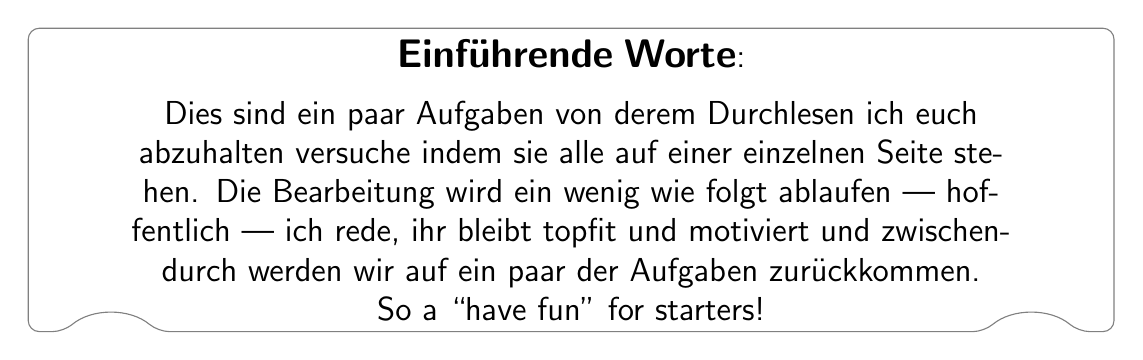
\begin{tikzpicture}
    \node[text width=13.5cm,align=center] (m) {%
        \textbf{\large Einführende Worte}:\medskip\\%
        Dies sind ein paar Aufgaben von derem Durchlesen ich euch abzuhalten versuche indem sie alle auf einer einzelnen Seite stehen. Die Bearbeitung wird ein wenig wie folgt ablaufen~--- hoffentlich~--- ich rede, ihr bleibt topfit und motiviert und zwischendurch werden wir auf ein paar der Aufgaben zurückkommen.\\
        So a \say{have fun} for starters!
    };
\pgfonlayer{background}
    \node[below,xshift=1.1cm,yshift=19.5pt,scale=.4] at(m.south west) {\usebox\pinguboxA};
    \node[below,xshift=-1cm,yshift=19.5pt,scale=.4] at(m.south east) {\usebox\pinguboxB};
    \draw[rounded corners,gray,fill=white] (m.north west) -- (m.north east) -- (m.south east) -- ++(-.45cm,0) to[bend right=40] ++(-1.2cm,0) -- ([xshift=1.65cm]m.south west) to[bend right=40] ++(-1.2cm,0) -- ++(-.45cm,0) -- cycle;
\endpgfonlayer
\end{tikzpicture}\vspace*{-\baselineskip}
\end{center}

\TaskBlock(Mittel)[7]{Leonardo-Zahlen}
Analysieren Sie den Algorithmus hinsichtlich seiner totalen Korrektheit im Bezug auf die Berechnung der Leonardo--Zahlen.
Weisen Sie dafür alle notwendigen Eigenschaften nach oder liefern Sie geeignete Gegenbeispiele.

Die Leonardo-Zahlen sind definiert als (für \(n \geq 0\)): \begin{equation*}
    L(0) = 1,~L(1) = 1\qquad L(n) = L(n - 1) + L(n - 2) + 1
\end{equation*}

\begin{plainjava}
public static long L(int n) {
    if(n == 0 || n == 1) return 1;
    int l1 = 1, l2 = 1;
    for(int i = 0; i < n - 1; i++) {
        int tmp = l1;
        l1 = l2;
        l2 = tmp + l2 + 1;
    }
    return l2;
}
\end{plainjava}

\clearpage
\TaskBlock(Schwer)[\(3+4+10\)]{Algorithmusanalyse}
Lesen Sie sich den Anforderungstext durch und bearbeiten Sie dann die drei folgenden Teilaufgaben.

{\itshape\fontspec{overlock} Guten Tag ich bin Besitzer eines Plätzchenladens. Dafür verwende ich verschiedene Mehle (Weizen oder Dinkel), verwende Zucker oder Süßungsmittel, sowie stets eine weitere Komponente (Kokos oder Zimt).

Da ich alle Plätzchen gleich gern habe, werde ich sie alle immer zum selben Preis verkaufen.
Geld an sich ist auch gar nicht das Problem, leider können mir meine Zulieferer immer nur eine begrenzte Menge (in Gramm) an den jeweiligen Stoffen zur Verfügung stellen~- die kann ich ihnen aber geben. Die habe ich.
Weiter habe ich pro Jahr immer eine handvoll an Rezepten, die immer eine bestimmte Anzahl eines Mehls, eines Süßungsstoffes und einer weiteren Komponente pro Plätzchen benötigen.

Auf der Basis hätte ich jetzt gerne eine Möglichkeit herauszufinden, wie ich insgesamt immer maximal viele Plätzchen aus den gegebenen Ressourcen und Rezepten backen kann.}

\begin{enumerate}[label=\alph*)]
    \item Führen Sie eine Problemspezifikation durch\vfill
    \item Führen Sie eine Problemabstraktion durch\vfill
    \item Entwickeln Sie einen Pseudocode-Algorithmus, welcher das Problem löst\vfill\vfill\vfill
\end{enumerate}


\clearpage
\TaskBlock(Leicht)[\(1+2+2+1\)]{Typidentifikation}

Bestimmen Sie für jeden der folgenden Java-Ausdrücke den Typ \textit{jedes Teilausdrucks}, sowie das Gesamtergebnis. Sie dürfen Rundungsprobleme der Sprache ignorieren:\vspace*{3em}
\begin{enumerate}[label=\alph*)]
    \itemsep8em
    \item \bjava{14  -  3D  *  2  /  12}
    \item \bjava{(char)  ((byte)  'a'  +  3)  +  " Sonne"}
    \item \bjava{14  -  2  +  (3  >  9  ||  true  ^  false  ?  "Hallo"  :  "Welt")}
    \item \bjava{7 / 2  -  3  *  2.5  +  2f}
\end{enumerate}


\clearpage
\TaskBlock(Leicht)[\(2+3+2+1\)]{Programmausgabe}
Betrachten Sie das folgende Java-Programm und geben Sie für die kommentierten Zeilen jeweils an, welche Ausgabe diese erzeugen (tragen Sie diese in die entsprechende Box \smash{\tikz[baseline=.135cm]\draw[gray,rounded corners=1pt](0,0) rectangle (.9cm,.35cm+.33\baselineskip);} ein).
Beschreiben Sie weiter kurz, warum die jeweilige Ausgabe zustande kommt, indem Sie die Werte der beteiligten Variablen erklären.

\begin{plainjava}
public class Example {
    public static int main;
    public static String a = "Hallo";

    public static void main(String[] args) {
        int a = 7;
        int b = 15;
        System.out.println(a + "; " + main); // i)
        {
            float main = 3 * b++;
            Example.a += b;
            System.out.println(b + "; " + main); // ii)
        }
        System.out.println(a + "; " + b + "; " + main); // iii)
        System.out.println(Example.a + "; " + Example.main); // iv)
    }
}
\end{plainjava}
\def\boxForUser{\smash{\tikz[baseline=.375cm]\draw[gray,rounded corners=1pt](0,0) rectangle (9.15cm,.85cm+.33\baselineskip);}}
\begin{enumerate}[label=\roman*)]
    \item \boxForUser\vfill
    \item \boxForUser\vfill
    \item \boxForUser\vfill
    \item \boxForUser\vfill
\end{enumerate}
\clearpage
\TaskBlock(Mittel)[\(5 + 4 + 3\)]{Kachelland}

\begin{wrapfigure}[7]{R}{.2\linewidth}
\vspace*{-1.33\topsep}\downsize\linewidth{
\begin{tikzpicture}
    \draw[clip] circle [radius=15];
    \draw (-15,-15) grid (15, 15);
% \pgfinterruptboundingbox
%     \fill[] (-30,-30) rectangle (30,30);
% \endpgfinterruptboundingbox
\end{tikzpicture}}
\end{wrapfigure}
Sie befinden sich in Kachelland, welches auf einem schachbrettartigen Feld geplant wurde.
Für diese Aufgabe betrachten wir die Fortbewegungskosten, die ein Charakter auf den jeweiligen Feldern hat, wobei wir zwei Formen des Transports unterscheiden: ohne Hilfsmittel und im Boot.
Auf diese Weise definieren wir für jede Kachel des zweidimensionalen Landes wie teuer es ist sie ohne Hilfsmittel, oder mit einem Boot, zu überqueren und geben eine Zeit in Minuten an.
Dafür verwenden wir ein Array mit zwei Elementen: \bjava{cell = \{:lan:foot:ran:, :lan:boat:ran:\}}.
Eine negative Zahl kennzeichnet, dass es unmöglich ist, das Feld mit dem Transportmittel zu überqueren.
Konstruieren Sie die folgenden drei Methoden in Java. Achten Sie auch auf die Rückseite, des Blattes: \begin{enumerate}
    \item \bjava{static int[][][] newLand(int width, int height)}\\
        Erschaffen Sie ein neues rechteckiges Kachelland mit den gegebenen Dimensionen, in dem kein Feld passierbar ist. Sie dürfen annehmen, dass weder \bjava{width} noch \bjava{height} negativ sind.
    \item \bjava{static boolean set(int[][][] board, int x, int y, int foot, int boat)}\\
        Setzt die Fortbewegungskosten des Feldes \((x, y)\) auf \bjava{\{:lan:foot:ran:, :lan:boat:ran:\}}.
        Prüfen Sie ob die Koordinaten auch wirklich auf dem Brett existieren und geben Sie über den \bjava{boolean} zurück, ob die Kosten tatsächlich gesetzt werden konnten.
    \item \bjava{static int costs(int[][][] board, int x, int y, boolean byBoat)}\\
        Geben Sie die Kosten des jeweiligen Feldes zurück. Dabei entscheide \bjava{byBoat}, ob die Kosten ohne Hilfsmittel (\bjava{byBoat=false}) oder in einem Boot (\bjava{byBoat=true}) von Interesse sind.
        Ist das Feld nicht auf dem Brett, so ist es per Konvention \say{nicht passierbar}.
\end{enumerate}
\begin{plainjava}
public class TileCountry {
    static int[][][] newLand(int width, int height) {
\end{plainjava}
\vfill
\begin{plainjava}
    }
// } :yields: Nächste Seite
\end{plainjava}
\clearpage
\begin{plainjava}
// Fortsetzung
// public class TileCountry {
    static boolean set(int[][][] board, int x, int y, int foot, int boat) {
\end{plainjava}
\vfill
\begin{plainjava}
    }

    static int costs(int[][][] board, int x, int y, boolean byBoat) {
\end{plainjava}
\vfill
\begin{plainjava}
    }
}
\end{plainjava}
\clearpage
\TaskBlock(Mittel)[\(4+4\)]{Schleifenspiel}
Im Folgenden finden Sie zwei Code-Ausschnitte. Schreiben Sie diese so um, dass sie nur noch Schleifen der angegebenen Art verwenden, ohne dass sich das Verhalten des Codes verändert. Dabei repräsentiert \bjava{k} eine natürliche Zahl (exklusive \(0\)), welche Sie nicht kennen.
\begin{enumerate}
    \item Verwenden Sie eine \bjava{do}-\bjava{while} Schleife:
\begin{plainjava}
int[] x = new int[]{17, 22, 13, 0};
for(int i = 0; i < x.length - k; i += 1) {
    System.out.println(x[i]);
}
\end{plainjava}\vfill
    \item Verwenden Sie eine \bjava{for}-Schleife:
\begin{plainjava}
int i = 1;
do {
    i *= k;
    k -= i;
} while(k >= 5);
System.out.println(i);
\end{plainjava}\vfill
\end{enumerate}
\clearpage
\TaskBlock(Mittel)[\(2+2+3+3\)]{Methodenverstehung}
Betrachten Sie das folgende Java-Programm und geben Sie für die kommentierten Zeilen jeweils die Werte der Variablen \bjava{a}, \bjava{b} und \bjava{c} an (tragen Sie diese in die entsprechende Box \smash{\tikz[baseline=.135cm]\draw[gray,rounded corners=1pt](0,0) rectangle (.9cm,.35cm+.33\baselineskip);} ein).
Erklären Sie die Ausgaben dabei durch eine kurze Erläuterung der beteiligten Java-Mechanismen. Relevant sind: \begin{inlist}
    \item Überladungen
    \item Seiteneffekte
    \item Überschattungen
    \item Standardwerte
\end{inlist}. Sie dürfen in ihrer Skizzierung die römischen Zahlen verwenden, um auf die Mechanismen hinzuweisen.

\hfill\llap{\smash{\raisebox{-\height}{\(\begin{array}{cc<{\to}c} \T{H} & & 72\\ \T{a} & & 97\\\T{l} & &108\\ o & & 111\end{array}\)}}}%
\begin{plainjava}
public class MethodExample {
   public static char a;
   public static int b = 5;
   public static int c = 3;

   static int x(int a) {
      a = a * a;
      return b + 2;
   }

   static int x(char[] b) {
      a += b[1];
      return b[0];
   }

   static String x() {
      String b = "Hallo";
      return b;
   }

   public static void main(String[] args) {
      // 1)
      String c = x();
      // 2)
      int temp = x(c.toCharArray());
      // 3)
      int b = x(temp);
      // 4)
   }
}
\end{plainjava}
\clearpage
\def\boxForUser{\smash{\tikz[baseline=.375cm]\draw[gray,rounded corners=1pt](0,0) rectangle (3.75cm,.85cm+.33\baselineskip);}}
\def\boxLine{a: \boxForUser\quad b: \boxForUser\quad c: \boxForUser}
\begin{enumerate}[label=\arabic*)]
    \item \boxLine\vfill
    \item \boxLine\vfill
    \item \boxLine\vfill
    \item \boxLine\vfill
\end{enumerate}
\clearpage
\TaskBlock(Leicht)[\(5\)]{Reverse}
Schreiben Sie eine Methode \bjava{static void reverse(int[] arr)} welche das übergebene Array umdreht, sodass das erste Elemente nun an letzter Stelle steht, das zweite an vorletzter Stelle,~\ldots\ und das letzte Element nun an erster Stelle steht.
\begin{plainjava}
static void reverse(int[] arr) {
\end{plainjava}
\vfill
\begin{plainjava}
}
\end{plainjava}
\clearpage
\TaskBlock(Mittel)[\(2 + 6\)]{Kameraszenario}
Im Folgenden sehen Sie das Grundgerüst einer Kameraklasse. Bearbeiten Sie die folgenden beiden Teilaufgaben,
welche aufeinander aufbauen. Sie dürfen keine (Java-)Ausnahmen verwenden.
\begin{enumerate}
    \item Schreiben Sie einen leeren Konstruktor, welcher die von Java zugewiesenen Standardwerte explizit initialisiert. Dieser Konstruktor soll nicht aus Code abseits der \bjava{Camera}-Klasse aufrufbar sein und so verhindern, dass weitere Kamera-Objekte erstellt werden können.
    \item Erweitern Sie die Klasse nun in sofern, dass es immer maximal fünf Kamera-Objekte gibt, welche durch \bjava{get(int)} durch eine Zahl \(x \in \{0, 1, 2, 3, 4\}\) abgefragt werden können. Dabei soll ein Kamera-Objekt erst (mit ihrem vorher erzeugten Konstruktor) erzeugt werden, wenn es durch die Zahl angefragt wird. Weiter sollen Folgeanfragen mit der Zahl dasselbe Objekt zurückliefern. Geben Sie für \(x < 0\) und \(x \geq 5\) den Wert \bjava{null} zurück.
\end{enumerate}
Falls Ihnen der Platz nicht reicht, markieren Sie bitte die Fortsetzung auf dem letzten Blatt.
\begin{plainjava}
public final class Camera {
   private int x, y, z;
   private boolean recording;
\end{plainjava}
\vfill
\begin{plainjava}
   public void move(int dx, int dy, int dz) { x += dx; y += dy; z += dz; }
   public void start() { this.recording = true; }
   public void stop() { this.recording = false; }
   public int[] position() { return new int[]{x, y, z}; }
   public boolean running() { return this.recording; }
}
\end{plainjava}
\clearpage
% \T{\color{gray}// Freie Seite als Platz für Aufgabe \thepage}
% \strut\clearpage
\TaskBlock(Mittel)[\(9\)]{Fehlersuche}
Im Code auf der nächsten Seite finden sich \textbf{10 Fehler}, welche vom Java-Compiler erkannt werden.
Identifizieren Sie \textbf{acht} dieser Fehler durch \begin{enumerate}
    \item die Angabe der Code-Zeilennummer und
    \item eine kurze Erklärung, was den Fehler verursacht.
\end{enumerate}
Tragen Sie die Informationen in die Tabelle ein.
Wenn Sie mehrere Fehler in einer Code-Zeile finden, tragen sie diese separat ein~--- die zusätzlichen Zeilen existieren dabei nur, um Ihnen eine Selbstkorrektur zu ermöglichen.
Folgefehler zählen dabei nicht als separate Fehler. Wird also beispielsweise ein Bezeichner inkorrekt initialisiert, so zählt nicht jede Verwendung als zusätzlicher Fehler sondern nur die inkorrekte Initialisierung.
\vfill
\def\arraystretch{1.85}
\begin{tabularx}{\linewidth}{rp{4em}X}
\toprule
    \# & Zeile & Grund\\
\midrule
    1 & & \\\midrule
    2 & & \\\midrule
    3 & & \\\midrule
    4 & & \\\midrule
    5 & & \\\midrule
    6 & & \\\midrule
    7 & & \\\midrule
    8 & & \\\midrule
    9 & & \\\midrule
   10 & & \\\midrule
   11 & & \\\midrule
   12 & & \\\midrule
   13 & & \\
\bottomrule
\end{tabularx}
\vfill
\clearpage\null\vfill
\lstset{lineskip=5.5pt}\lstcolorlet{numbers}{black}
\begin{plainvoid}[numbers=left,numbersep=6pt]
public class iDoGood {
    final void i = 0x7;
    private final String omega = "Sunshine";

    static int iMultiply(final char x, double y) {
        return x * y;
    }

    public IDoGood(String dromeda) {
        this.omega = dromeda;
    }

    static int double(byte i) {
        return 2 * ++i;
    }

    private iDoGood() {
        this(andromeda);
    }

    private boolean iDoGood() {
        if(this.omega.equals("andromeda"));
        int i = 0 // /** // **/ /* ;
        for(;i < 2_00;i++, i += 2)
            System.Err.println(i);
        return false /** // */ ;
    }

    static class iDoBetta {
        global doBetta() {
            iDoGood veryGud = iDoGood();
            System.out.println(veryGud.omega);
        }
    }
}
\end{plainvoid}
\vfill\null
\clearpage
\T{\color{gray}// Freie Seite als zusätzlicher Platz}
\strut
\end{document}